%%% The ``\documentclass'' command has one parameter, based on the kind of
%%% document you are preparing.
%%%
%%% [annual] - Technical paper accepted for presentation at the ACM SIGGRAPH 
%%%   or SIGGRAPH Asia annual conference.
%%% [sponsored] - Short or full-length technical paper accepted for 
%%%   presentation at an event sponsored by ACM SIGGRAPH
%%%   (but not the annual conference Technical Papers program).
%%% [abstract] - A one-page abstract of your accepted content
%%%   (Technical Sketches, Posters, Emerging Technologies, etc.). 
%%%   Content greater than one page in length should use the "[sponsored]"
%%%   parameter.
%%% [preprint] - A preprint version of your final content.
%%% [review] - A technical paper submitted for review. Includes line
%%%   numbers and anonymization of author and affiliation information.

\documentclass[annual]{acmsiggraph}

\usepackage[usenames]{color}
\newcommand{\CD}[1]{{\color{magenta}{\textbf{CD: #1}}}}


%%% If you are submitting your paper to one of our annual conferences - the 
%%% ACM SIGGRAPH conference held in North America, or the SIGGRAPH Asia 
%%% conference held in Southeast Asia - there are several commands you should 
%%% consider using in the preparation of your document.

%%% 1. ``\TOGonlineID''
%%% When you submit your paper for review, please use the ``\TOGonlineID''
%%% command to include the online ID value assigned to your paper by the
%%% submission management system. Replace '45678' with the value you were
%%% assigned.

\TOGonlineid{45678}

%%% 2. ``\TOGvolume'' and ``\TOGnumber''
%%% If you are preparing a preprint of your accepted paper, and your paper
%%% will be published in an issue of the ACM ``Transactions on Graphics''
%%% journal, replace the ``0'' values in the commands below with the correct
%%% volume and number values for that issue - you'll get them before your
%%% final paper is due.

\TOGvolume{0}
\TOGnumber{0}

%%% 3. ``TOGarticleDOI''
%%% The ``TOGarticleDOI'' command accepts the DOI information provided to you
%%% during production, and which makes up the URLs which identifies the ACM
%%% article page and direct PDF link in the ACM Digital Library.
%%% Replace ``1111111.2222222'' with the values you are given.

\TOGarticleDOI{1111111.2222222}

%%% 4. ``\TOGprojectURL'', ``\TOGvideoURL'', ``\TOGdataURL'', ``\TOGcodeURL''
%%% If you would like to include links to personal repositories for auxiliary
%%% material related your research contribution, you may use one or more of
%%% these commands to define an appropriate URL. The ``\TOGlinkslist'' command
%%% found just before the first section of your document will add hyperlinked
%%% icons to your document, in addition to hyperlinked icons which point to
%%% the ACM Digital Library article page and the ACM Digital Library-held PDF.

\TOGprojectURL{}
\TOGvideoURL{}
\TOGdataURL{}
\TOGcodeURL{}

%%% Replace ``PAPER TEMPLATE TITLE'' with the title of your paper or abstract.

\title{Interactive simulation of surgical suturing}

%%% The ``\author{}'' command takes the names and affiliations of each of the
%%% authors of your paper or abstract. The ``\thanks{}'' command takes the
%%% contact information for each author.
%%% For multiple authors, separate each author's information by the ``\and''
%%% command.

\author{Anonymous}

%%% The ``pdfauthor'' command accepts the authors of the work,
%%% comma-delimited, and adds this information to the PDF metadata.

\pdfauthor{Anonymous}

%%% Keywords that describe your work. The ``\keywordlist'' command will print
%%% them out.

\keywords{Suture simulation, knot tying, constraints, compliance computation, haptic feedback}

%%% The ``\begin{document}'' command is the start of the document.

%%% If you have user-defined macros, you may include them here.

% example of a user-defined macro called ``remark.''
% \newcommand{\remark}[1]{\textcolor{red}{#1}}

\begin{document}

%%% A ``teaser'' image appears under the title and affiliation information,
%%% horizontally centered, and above the two columns of text. This is OPTIONAL.
%%% If you choose to have a ``teaser'' image, it needs to be placed between
%%% ``\begin{document}'' and ``\maketitle.''

%\teaser{
%   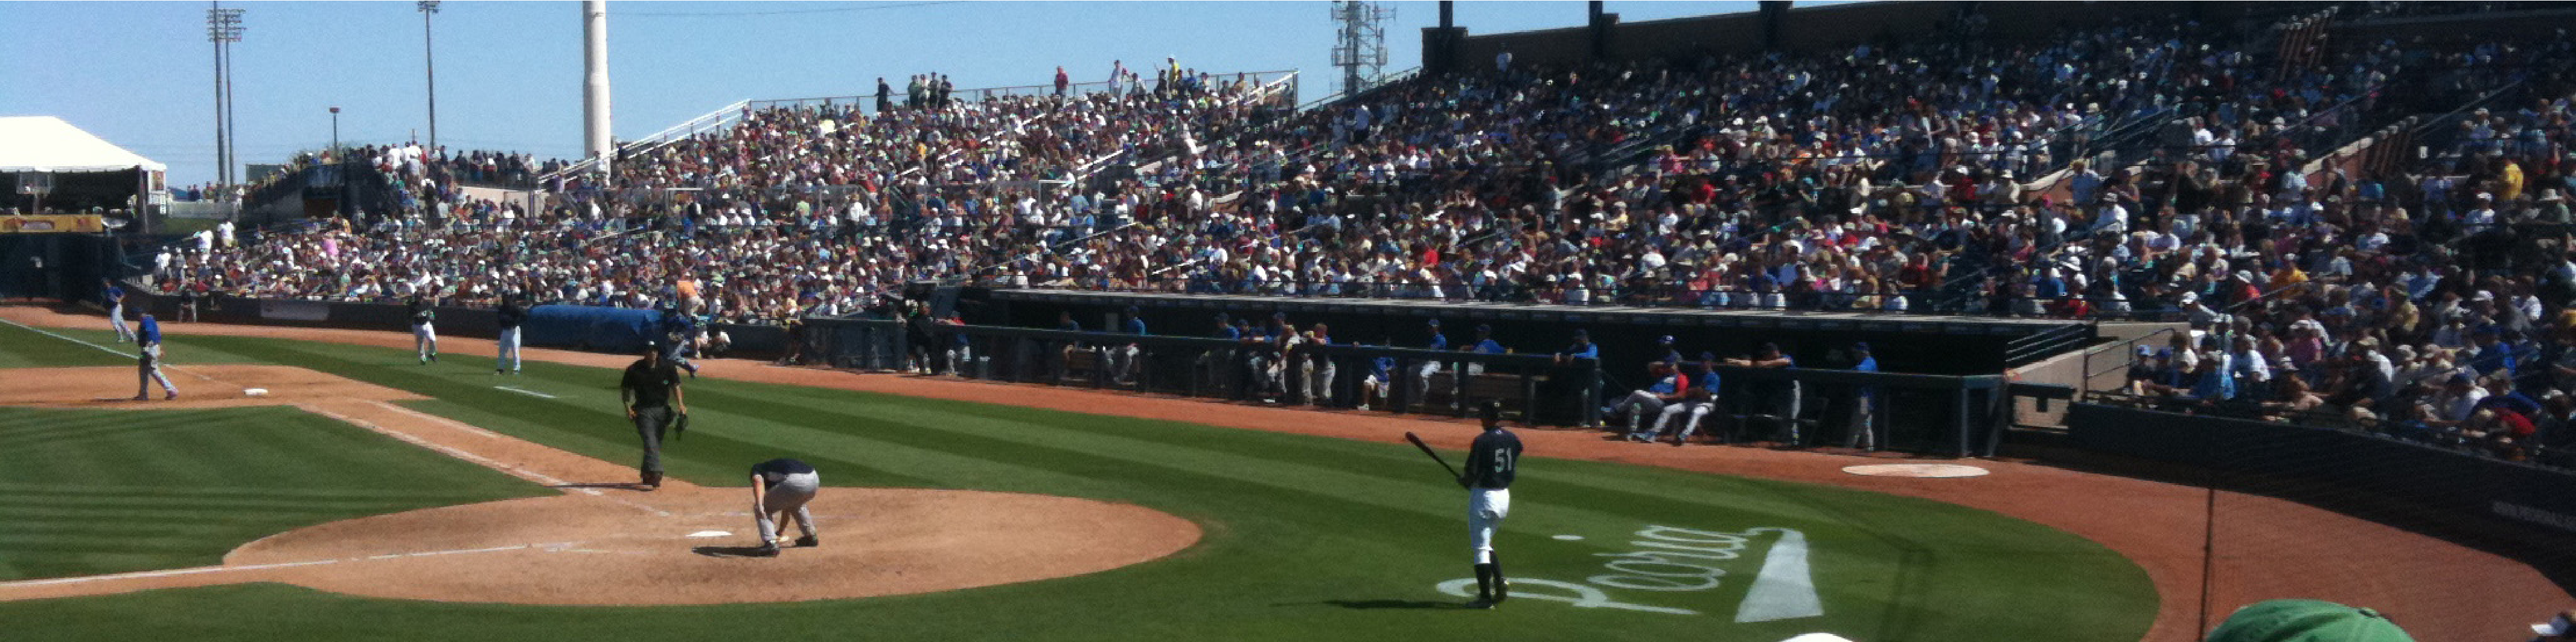
\includegraphics[height=1.5in]{images/sampleteaser}
%   \caption{Spring Training 2009, Peoria, AZ.}
%}

%%% The ``\maketitle'' command must appear after ``\begin{document}'' and,
%%% if you have one, after the definition of your ``teaser'' image, and
%%% before the first ``\section'' command.

\maketitle

%%% Your paper's abstract goes in its own section.

\begin{abstract}

This paper introduces algorithms for simulating suturing of deformable tissues.
\textit{(1) Importance of the clinical aspects 
(2) What are the "key" of the a good suture.}

Our interactive simulation :
(1) accurately simulates the behavior the thread 
(2) models the coupling between the thread and the deformable tissue
(3) stable behavior using implicit integration
(4) allows for haptic feedback

Our Contributions are
(1) A novel algorithm for automatic and adaptive sampling of FEM beam elements 
(2) An optimized constraint-based approach for suture simulation
(3) GPU Preconditionner approach for solving the constraints accurately and quickly
(4) ? Haptic Feedback based on an asynchronous recomputation of the constraints (not very new...) 

\end{abstract}

%%% ACM Computing Review (CR) categories.
%%% See <http://www.acm.org/class/1998/> for details.
%%% The ``\CRcat'' command takes four arguments.

\begin{CRcatlist}
  \CRcat{I.3.5}{Computer Graphics}{Computational Geometry and Object Modeling}{Physically based modeling};
   \CRcat{I.3.7}{Computer Graphics}{Three-Dimensional Graphics and Realism}{Animation};
   \CRcat{I.6.8}{Simulation and Modeling}{Types of Simulation}{Animation};  
    \CRcat{I.6.8}{User Interfaces}{Haptic I/O};   
\end{CRcatlist}

%%% The ``\keywordlist'' command prints out the keywords.

\keywordlist

%%% The ``\TOGlinkslist'' command will insert hyperlinked icon(s) to your
%%% paper. This includes, at a minimum, hyperlinked icons to the ACM article
%%% page and the ACM Digital Library-held PDF. If you added URLs to
%%% ``\TOGprojectURL'' or the other, similar commands, they will be added to
%%% the list of icons.
%%% Note: this functionality only works for annual-conference papers.

%\TOGlinkslist

%%% The ``\copyrightspace'' command 
%%% Do not remove this command.

\copyrightspace

%%% This is the first section of the body of your paper.

%%%%%%%% %%%%%%%%
%%  SECTION : Introduction   %%
%%%%%%%% %%%%%%%%

\section{Introduction}

\paragraph{Motivations}

Suturing is one of the most common tasks in surgery. (d�tailler). -Quand on l?apprend (early stage of the surgery eduction) - 
Comment ne pas �rater� une suture ?

However, the increasing complexity of surgical procedure, and particularly for minimally invasive surgery (MIS) may (rendre + difficile) the achievement of a suture.

For example, during a laparoscopic procedure, the surgeon does not have a direct view on the operative field. They execute the suture using graspers while controlling their gesture using a camera.

Hence, the students in surgery do extensive training for acquiring this so-called ?basic skills? for MIS. Commercial training simulators already propose suturing simulations in their ?basic skills? modules but the results are not yet realistic.

\paragraph{Difficulties}

\begin{itemize}
\item Various type of interactions:
Contacts (sometimes very constrained like knot tying), insertion inside the tissue, friction,  - Needle : rigid / Thread :flexible 
\item Coupling between two very different deformable models => tissue (low stiffness, high mass) and thread (high stifness, low mass)"
\item Maintaining a stable simulation and compatible with haptic rendering.
\end{itemize}

\paragraph{Our Method}
To adress these challenges, we introduce:
\begin{itemize}
\item n adaptive beam model with automatic sampling based on the curvature. Coupled with  Bloc -Tri-Diagonal (BTD) solver for O(n) computation of the deformation (n= number of node)
\item A constraint-based approach for modeling the suture: a set of dedicated constraint, based on complementarity for modeling the different stages of the suture procedure. 
\item For solving these constraints, the mechanical coupling between the suture model and the soft-tissue model is physically modelled using compliance. Two different strategies are used for the soft-tissue and the surgical thread. The compliance of the soft-tissue is approximated using an asynchronous preconditionner that is factorized in a separated thread and solved in real-time with a GPU strategy. 
For the suture model, compliance is not fully built and an optimization based on the BTD Solver is used.
\item The time integration relies on implicit euler with quite large time steps. The haptic rendering is based on an asynchronous re-computation of the constraints which is similar to \cite{PNDCK11}.
\end{itemize}


%%%%%%%% %%%%%%%%%
%%  SECTION : Related Work   %%
%%%%%%%% %%%%%%%%%

\section{Related Works: copy paste from a -never published- paper}
\label{sec:previous}
There are many areas of interest for the simulation of a suturing task. Deformations models are needed for the soft tissue, the needle and the surgical thread. A fast and physically correct method for the interaction of the suture with the tissue has to be devised. 

% tissue model
Regarding the simulation of the deformation of soft tissue, it is key that the model can capture the geometrical non-linearities that take place during the manipulation of the tissue or its interaction with the needle. Such models have been proposed in the context of suturing tasks, some of them based on real-time implementations of the Finite Element Method \cite{Berkley04,Holbrey04} but a majority uses mass-spring systems \cite{Marshall05,Zhang07,Wang08,Shi08} for their simplicity and computational efficiency.

% suture model
%  geometrical approaches
Suture and surgical threads have often been modeled as an articulated object composed of linear links connecting spherical joints \cite{Brown04,Marshall05,Zhang07}, where the thread motion is controlled by a \textit{follow the leader} approach.
%  mass-springs
Phillips \textit{et al.} \cite{Phillips02} model a rope by creating a spline of overlapping spheres representing mass-points connected by simple springs. More advanced "springs" functions have been added to account for bending and twisting in \cite{Wang05}. 
%  Cosserat rods
Pai \cite{Pai02} proposed a model based on Cosserat rods which expresses the configuration of thin elastic solids as a boundary value problem. The approach is physically correct but does not handle dynamics. Bertails \textit{et al.} \cite{Bertails09} improved on this model by achieving linear complexity with respect to the number of vertices used for the discretization. Spillman and Teschner \cite{Spillmann07} introduced dynamics to the model and made the rod behaviour independant of the underlying discretization. With the observation that the twisting wave travels faster through the rod than the compression, Bergou \textit{et al.} \cite{Bergou08} further improved the computation time.
%  splines
Lenoir \textit{et al.} \cite{Lenoir02} used dynamic Lagrangian splines to model a surgical thread which can be constrained by Langrangian multipliers. They added \textit{sliding point} constraints with friction \cite{Lenoir04} to simulate suturing tasks. However the model does not incorporate twisting energy, thus limiting its range of applications. This was later improved by Theetten \textit{et al.} \cite{Theetten08} who proposed a geometrically exact spline model which can account for twist, both for dynamic and quasi-static simulations.

%  knots
Knots tying is an important aspect of the medical suturing procedures and requires tedious learning. Previous works extensively studied the interaction required for knot-tying \cite{Phillips02,Lenoir02,Spillmann08}. Suture simulations integrating such capability of tying knots with surgical thread are described in \cite{Brown04,Marshall05,Shi08} for instance. These approaches either do not use physically-based deformable models, or lower their accuracy in order to achieve interactive rates.

% needle model
When considering needles in the context of suturing, the assumption is made that the needle is rigid. This assumption is not always valid, such as within new endoscopic surgical techniques (NOTES\footnote{NOTES: Natural Orifice Transluminal Endoscopic Surgery}), suturing tasks should thus also consider flexible needles. A certain amount of previous work can be found in the area of needle biopsy simulation or brachytherapy simulation for instance. Dimaio and Salcudean \cite{DiMaioSalcudean03} modeled a flexible needle with two-dimensional triangular elements and used a nonlinear finite element method to compute the needle's deformation. Later simulations use three-dimensional flexible needles \cite{DiMaio05}. Several studies have also proposed models for flexible needles to study needle steering \cite{Abolhassani07b,Chentanez09}. 

% needle interaction + suture interaction
Regarding the interaction of the needle with soft tissues, a recent survey by Abolhassani \textit{et al.} \cite{Abolhassani07} summarizes existing methods, however the referenced works do not consider suturing. In general, the interaction between needle and tissue combines different physical phenomena. Three different forces are often associated to the insertion of a needle in soft tissues: puncture force, cutting force and friction force. Several studies have identified these forces through a series of experiments \cite{Simone02,Okamura04}, and were used to parameterize existing models \cite{Crouch05,Dehghan08}. As for previous work directly related to suturing simulation, LeDuc \textit{et al.} \cite{LeDuc03} proposed an interaction model where the suture can pierce the mesh only at vertices, which can then slide with friction from one suture node to the next. Similar approaches were used in later studies by \cite{Zhang07}.
Nageotte \textit{et al.} \cite{Nageotte05} build a path planner based solely on a geometrical modeling of a suturing task. A few other works consider the subdivision of the mesh at the collision point \cite{Marshall05, Shi08}. Finally, Lenoir \textit{et al.} \cite{Lenoir04} used \textit{sliding point} constraints with friction solved by Lagrangian multipliers to simulate the interaction between the suture and the organ. An active set strategy required multiple solving passes until the status of all the constraints is determined.
%
% siggraph09 paper
%The method we propose uses complementarity constraints to describe the interaction between soft-tissues and medical devices. As such it differs significantly from previous works that typically rely on force models to describe the interaction. To our knowledge, the only work to share some similarities with our method is the one recently proposed by Chentanez \textit{et al.} \cite{Chentanez09} for the simulation of needle insertion. Yet, it differs on multiple aspects: in particular our method does not require remeshing or reparameterization along the path of the needle, and we can significantly reduce the cost of the Jocabian matrices involved in the computation through the use of a technique called {\rm Compliance Warping} introduced by Saupin \textit{et al.} \cite{Saupin2008}. Also, while Chentanez \textit{et al.}  guess the status of the constraints in a \textit{active sets strategy} manner and need to solve multiple conjugate gradients before finding the correct configuration, we solve the linear complementary problem using only one run of a Gauss-Seidel algorithm, where constraints can change status between each iteration. 
%
Recently, a similar idea was proposed by Chentanez \textit{et al.} \cite{Chentanez09} to model the interaction between a soft tissue and a flexible needle using stick slip friction. They  guess the status of the constraints in a \textit{active sets strategy} manner and need to solve multiple conjugate gradients before finding the correct configuration. 

% contraintes
Complementarity constraints have been used by Duriez \textit{et al.} \cite{Duriez06} for the simulation of the interaction of deformable models. The resolution of the system is based on the Gauss-Seidel algorithm which is quite common when solving a linear complementarity problem (see \cite{Cottle,Jourdan98,Erleben07,Otaduy09}). The use of distributed constraints have been discussed by Sifakis \textit{et al.} \cite{Sifakis07}, and a framework allowing the use of heterogeneous constraints is a simulation has been introduced by Gu\'ebert \textit{et al.} \cite{Guebert08}.

In the following sections, we show how we generalize the use of complementarity constraints (that are not limited to contact and friction) to account for the numerous types of interaction that takes place during suture (contact between the tissue walls, self-collision of the thread, puncture of the needle inside the tissue, cutting through different layers,... ). Then we propose to solve the  complementarity problem without \textit{active sets} using only one run of a Gauss-Seidel algorithm, where the constraints can change status between each iteration. 



%%%%%%%% %%%%%%%%%%%
%%  SECTION : Adaptive Beams   %%
%%%%%%%% %%%%%%%%%%%
\section{Adaptive Beams model for the suture}

Motivation: Modeling accurate deformation with large displacement  + stable + knot tying + rigidifications + fast + allow constraints with the grasper + (elongation constraints) 

Solution: Model based on the beam theory but with an adaptive sampling based on the curvature => allows for knot tying without excessive sampling. In a real-time context, when the node is "tighten", we propose to "rigidify" the node (i.e. the knot has a behavior of a rigid body).

\subsection{Finite Element Method based on beam theory}
\CD{Copy-paste of a previous paper:}
In this work, we use a model that relies on beam theory and can handle deformations with large displacements.
The model itself is not part of our contribution as it has been extensively used in the field of computational mechanics and has already been introduced  by Cotin \textit{et al.} \cite{Cotin05} in the context of medical simulation. However, this study shows that a model consisting of serially-linked beam elements is perfectly suitable for both needle and thread, even if their mechanical properties are different, by adjusting the parameters of the beams.

A beam model describes the deformation of a curve representing the neutral fiber of the deformation stress. It is assumed to be discretized by a series of nodes linked by beam elements. Each node is associated to a reference frame so that the deformation of each beam element is computed locally in this frame using linear elasticity. As such the model allows for small deformations but large displacements, which suits well this type of application. Each beam is capable of resisting axial forces, bending moments about the two principal axes in the plane of its cross section, and twisting moments about its centroidal axis. Details about the beam models can be found in several books, such as \cite{Przemieniecki}.

An advantage of using this model is that we can parametrize it to either describe a nearly rigid object (i.e. a needle) or a very soft object (i.e. a surgical thread). Parameters affecting the behavior are: $E$, the Young Modulus, $\nu$ the poisson ratio, $A$ Area of the cross section and $\rho$ the density. The computation of serially-linked beam elements can be optimized using a Band Tri-Diagonal solver which enables real-time simulation of the deformation of models up to several hundreds elements.


\subsection{Adaptive sampling of the beam elements}

Motivation: During knot tightening, the thread undergoes important deformations very locally but not everywhere. 
It means that the sampling of the beams must be dense at the node location. 
This location can not be predefined, as the user may tighten the node at any curvilinear abscissa of the thread model.
An homogeneous dense sampling of the beams is not 



%%%%%%%% %%%%%%%%
%%  SECTION : constraints   %%
%%%%%%%% %%%%%%%%

\section{Constraint-based interaction model \CD{Copy-paste of a previous paper: A RACCOURCIR ?}}

\label{sec:constraints}

Our main contribution in this study is a new interaction model to describe the mechanical phenomena occuring during suturing tasks. For the interaction model, our approach relies on complementarity theory to describe the interactions between the needle or surgical thread and the soft tissue during a suturing procedure. Complementarity theory relies on the use of certain pairs of inequality constraints that are complementary, in the sense that at least one must hold with equality. In this section, we present a toolbox of constraints for the different aspects of the interaction. 


\subsection{Methodology}
The following notations are used: $\delta$ is a measure of a distance between a current state and a target state that will be redefined for each constraint. $\lambda$ represents the force used to solve the constraint (applied by the tissue on the needle or the thread). In general, $\delta$ and $\lambda$ are both unknown.
We assume that the mechanical model of the interacting objects could provide a linearized law between them:
\begin{equation}
\label{complianceLaw}
\delta(\lambda) =  \mathbf{W}\lambda + \delta_0
\end{equation}
where $\mathbf{W}$ is a compliance measure and $\delta_0$ the value of $\delta$ when $\lambda$ vanishes to zero. This law is called the \textit{compliance law}. 
% A relire :
It must be noted that if the constraint is of dimension 1, the terms of this equation are scalars. However, should the constraint be of higher dimension (e.g. friction constraint), $\mathbf{W}$ is a small matrix, usually $3\times3$, and $\delta$ is a vector.
%
Each constraint defines another law between $\delta$ and $\lambda$, called the \textit{constraint law}. 
As we know the two laws, the unknown values of $\lambda$ and $\delta$ can be generally computed easily. 
However, all constraints are coupled and we will see in section \ref{subsec:resolution} that $\delta_0$ value depends on other constraints and asks for an iterative approach during the global solving process. 

In this section, we suppose that $\delta_0$ is known so that we can explain each constraint independantly. 
In particular, the following paragraphs details the different \textit{constraint laws} used by our method.


\subsection{Puncturing soft tissue}

A first type of complementarity constraint was designed specifically to model the interaction between the needle tip and the tissue.
This model can capture accurately the physical transient states when the needle penetrates (and puctures) the soft tissue. 
We identify three possible states (no contact, active contact, penetration) which are defined with a set of inequalities, as illustrated in Fig. \ref{puncturing}. We define $\delta_p = (Q-P).\vec{n}$, with $Q$ the tip of the needle, $P$ the collision point and $n$ the surface normal vector at point $P$. % given by a continuous collision detection method
%
\begin{figure}[htbp]
\centering
   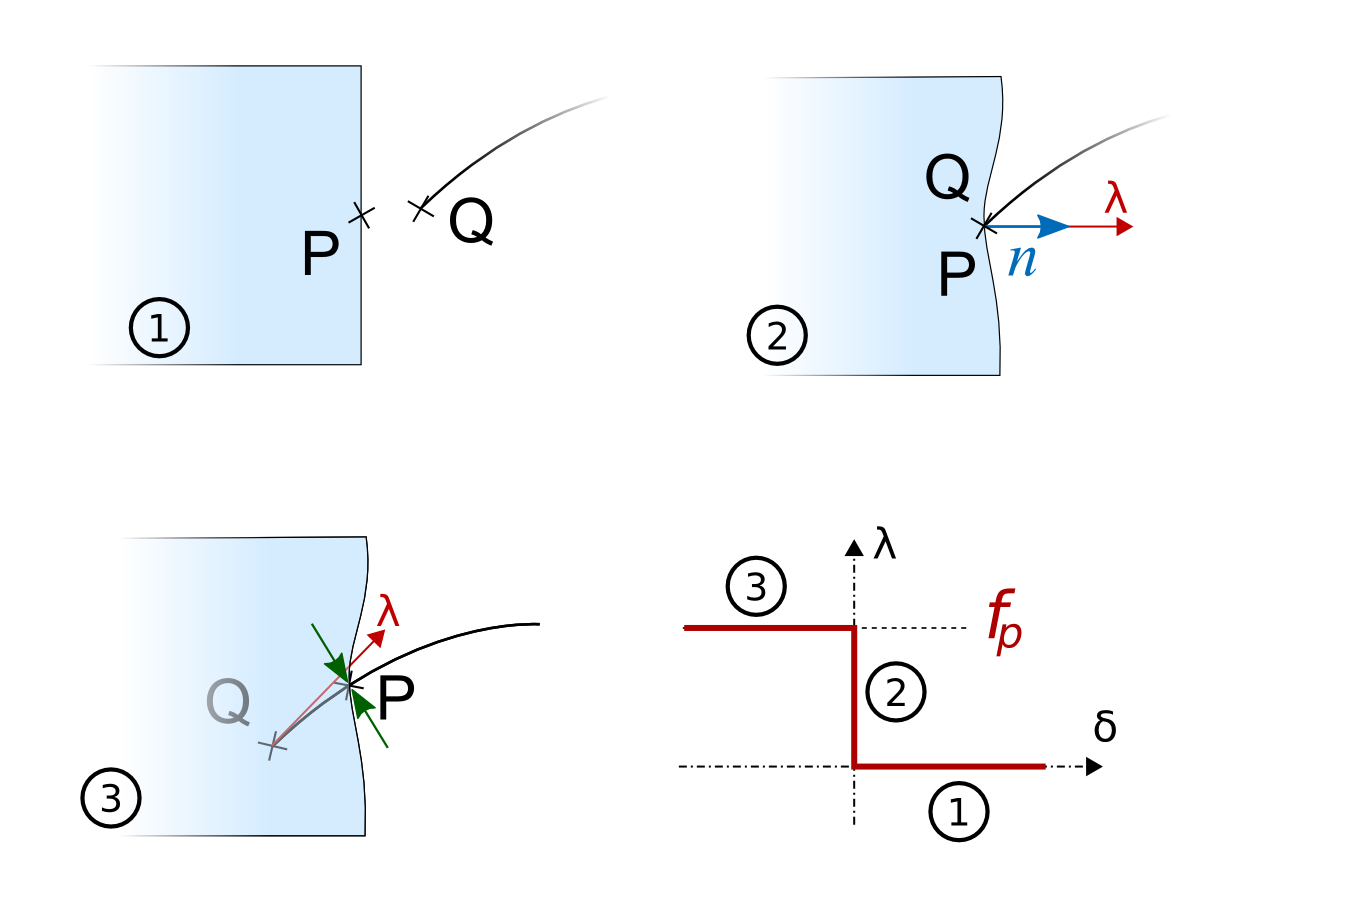
\includegraphics[width=10cm]{IMG/Puncture.png}
   \caption{(1) The needle moves freely in space, (2) the needle collides with the surface of the soft tissue, resulting in a contact force normal to the surface of the soft tissue, and (3) the needle punctures the soft tissue, resulting in a contact force in the direction of the needle shaft.
Similarly to the coulomb's law, the solution is found by an intersection of the line given by the \textit{compliance law} and the graph of the constraint.} 
\label{puncturing}
\end{figure}
%
When the needle-tip collides the soft-tissue wall, the constraint tries first to prevent the interpenetration, as a contact constraint. However, when the interaction force $\lambda$ reaches a puncturing force threshold $f_p$, the needle starts penetrating through the soft tissue as depicted in Fig. \ref{puncturing}. 
% Ajout depuis SCA :
The constraint law can be written with two complementarities:
\begin{equation}
\left\{
\begin{array}{l}
0 \leq \delta_p \perp  \lambda_p \geq 0   \  \mathrm{if} \   \lambda_p< f_p \\
0 \leq - \delta_p \perp  f_p - \lambda_p \geq 0  \  \mathrm{if}  \   \lambda_p > 0 
\end{array}
\right.
\end{equation}

If equation (\ref{complianceLaw}) is available (when discoupled from other constraint), the resolution is quite straightforward:

% ALGO
% if(delta_0 > 0)
%    return lambda = 0
% else
%	lambda = delta_0/W
%      if (lambda < f_p)
%		return lambda
%      else
%		lambda = f_p
%		return lambda

\vspace{1cm}

\textbf{ALGO}

\vspace{1cm}

%This expression is not compatible with standard Linear Complementarity Problem (LCP) solvers.  
%It has to be "augmented" by introducing a new parameter $d$ that represents the norm of the relative displacement, when it is not null.
%\begin{equation}
%\left\{
%\begin{array}{l}
%0 \leq d+ \delta_p \perp  \lambda^{(1)}_p \geq 0   \\
%0 \leq d - \delta_p \perp  f_p - \lambda^{(2)}_p \geq 0 \\
%0 \leq d  \perp \lambda^{(1)}_p  +  f_p - \lambda^{(2)}_p  \geq 0 \\
%\end{array}
%\right.
%\end{equation}
%where $\lambda_p =  \lambda^{(1)}_p+ \lambda^{(2)}_p$ .




%The resolution is straightforward and consists in adding the puncture test to a contact constraint : if $\lambda_p > f_p$ then $\lambda_p = f_p$.
%%%%%% C'est quoi ce truc ?

\begin{figure}[htbp]
\centering
   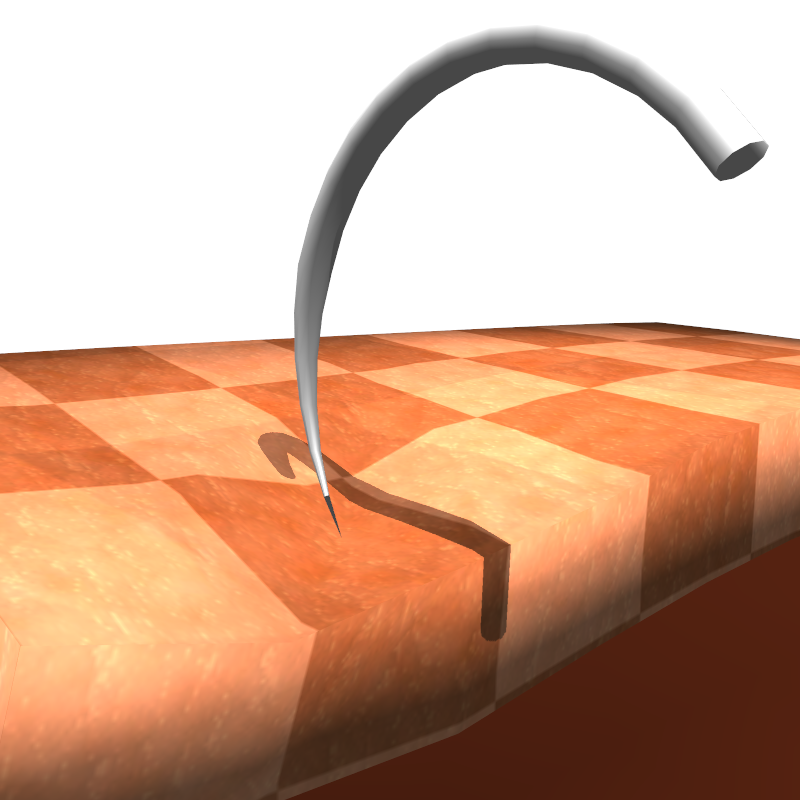
\includegraphics[width=4cm]{IMG/PunctureConstraint2.png}
   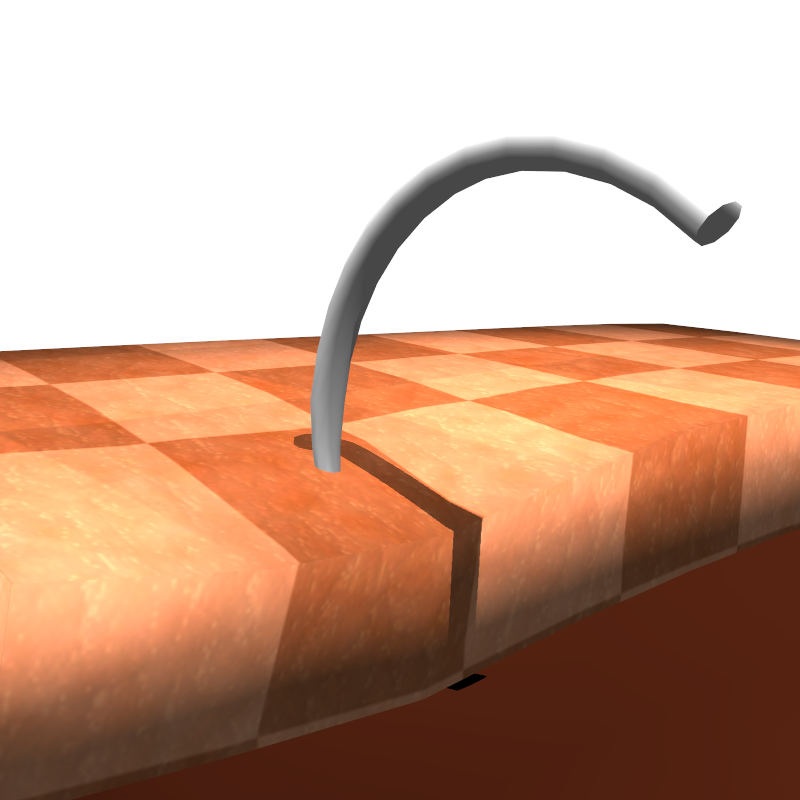
\includegraphics[width=4cm]{IMG/PunctureConstraint3.png}
   \caption{Puncturing steps: contact is activated first and when the threshold is reached, the needle penetrates. } 
\label{puncturing2}
\end{figure}
%
The force threshold $f_p$ has been studied for needle insertion simulations \cite{Simone02}, and it has been shown that its magnitude depends on the needle tip design and the material properties of the tissue being punctured. A membrane effect is very common, where the resistance of the surface is sensibly larger than deeper tissue layers. Our approach also allows the simulation of the insertion of the needle through a non-homogeneous structure composed of multiple layers, such as the skin for which we identify the dermis and the epidermis. We apply several puncture constraints during the simulation, at each tissue layer encountered by the needle. It is possible to provide different values for the threshold force $f_p$ in order to model different tissue behaviors.

When the needle tip is in contact with the tissue, lateral motion is also constrained by friction constraints in the directions tangent to the surface. However, if the needle penetrates the tissue we impose a null relative displacement $\delta_n$ between the needle and the organ along the directions normal to the needle shaft. 
%
That is, the needle can slide through the puncture point but its lateral motion is constrained. Directions of the lateral constraints are dynamically updated during the constraints resolution if we see a change in the state of the puncture constraint.

\subsection{Cutting through soft tissues}

As the needle penetrates through the tissue, it encounters a certain resistance from the material slowing down its motion. The same effect applies on the surgical thread attached to the needle. Two separate forces have been identified : a friction occuring along all the needle shaft or along the thread (section \ref{sub:friction}), and a cutting force applied at the tip of the needle. 
%This cutting force is considered to include a combination of the plastic deformation from the act of cutting and the tissue stiffness at the tip of the needle, since the tissue is compressed in front of the cuts. 

For the needle to cut through the tissue and move forward, the force applied to the needle by the user or the tool needs to overcome this cutting force. If this threshold is not reached, the tip can still move as it will compress the tissue without cutting it. Of course, if the needle is retracted, no force is applied to the tip. We model this behavior by a constraint very similar to the one used for puncturing, except that in this case the gap $\delta$ is the relative displacement between the needle tip and the end of the recorded needle path. This enables us to simulate the fact that no cutting force is applied if the needle is re-inserted at the same location and following the same path. The magnitude of the cutting force threshold $f_c$ can be extracted from experimental data, which often show that the cutting force is less than the puncture force $f_p$. If the tissue is homogeneous the cutting force is constant throughout all the tissue. However, as for $f_p$ it can be tuned to different values from a tissue layer to another. The resolution of this constraint and its constraint law are similar to the ones defined for the puncture constraint, in the direction of the needle.

\subsection{Suture path through soft tissues}

To generalize our approach and have a more consistent behavior when inserting either the needle of the thread through the tissue, we use the same deformable model for the needle and the suture (see section \ref{sec:defmodel} for a description of the model). Therefore the interaction model considers only one model which is parameterized differently along the curve defined by the needle and surgical thread. This means that constraints created for the insertion of the needle are not modified when the suture starts sliding through the tissue. In this subsection and the next, we describe the interaction between the tissue and the composite model describing both the needle shaft and the surgical thread.

\begin{figure}[ht]
\begin{center}
    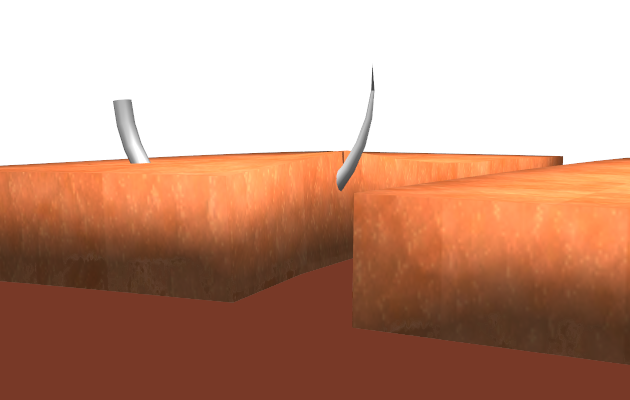
\includegraphics[width=4cm]{IMG/TipPath2.png}
    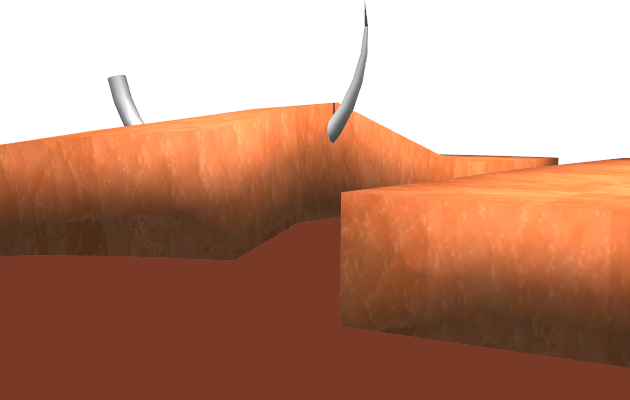
\includegraphics[width=4cm]{IMG/TipPath3.png}
   \caption{After insertion in the tissue, the needle is moved up: the constraints ensure that the tissue deformation follows the needle motion.}
\end{center} 
\label{needle_path}
\end{figure}

During the navigation of the needle and thread through soft tissues, we constrain the motion so that the needle and thread do not move laterally. For thus we use bilateral constraints to ensure that the needle shaft and thread stay in the path created by the needle tip. This is achieved by imposing a null relative displacement $\delta=0$ along the directions normal to the needle-thread curve.
Then, $\lambda$ is found using the \textit{compliance law} : $\lambda = -\delta_0 \mathbf{W}^{-1}$.

Constraints are sampled along the path of the needle-thread curve as described in section \ref{sub:sampling} and are created within the mesh describing the soft tissue and are static relatively to the motion of the surrounding tissue elements. At each time step, we look for the segment of the  discretized needle-thread model closest to the constraint point in the mesh, compute its direction and create two bilateral constraints in directions perpendicular to the segment. If the needle is retracted, we delete constraints as required. This allows the needle to be re-inserted along the same path or a completely different one.

\subsection{Friction}
\label{sub:friction}

When moving inside the tissue, the needle and surgical thread are slowed down by friction due to the tissue. We model dry friction in the tangential direction of the suture path curve using a complementarity constraint. This constraint consists of two states: static friction when there is no relative motion between the two objects that stick together and dynamic friction when the thread slip inside the tissue (Fig. \ref{fig:friction}). 
%
\begin{figure}[ht]
\begin{center} 
   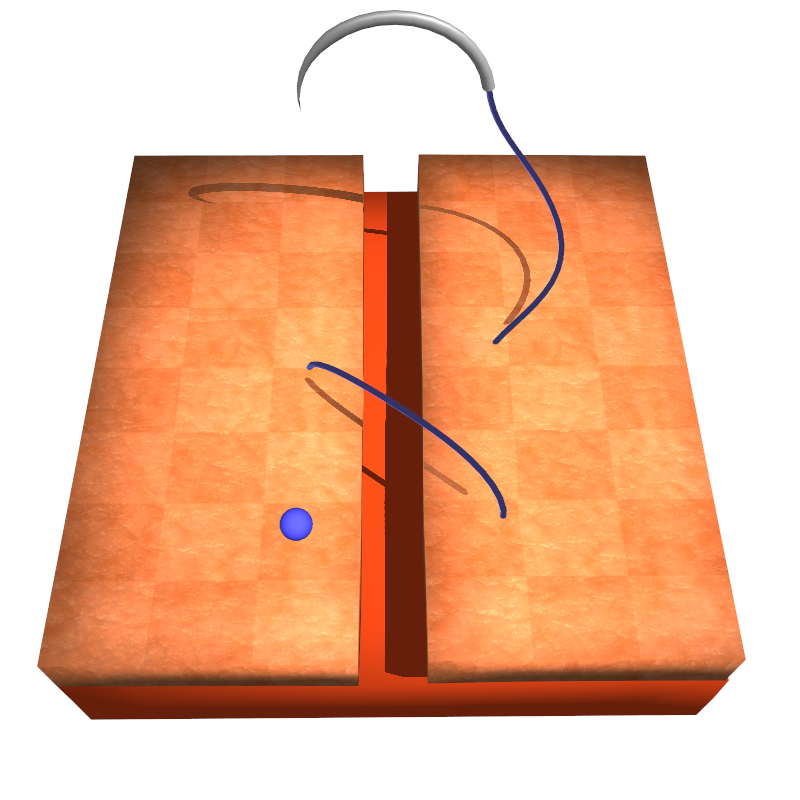
\includegraphics[width=4cm]{IMG/FrictionConstraint1.png}
   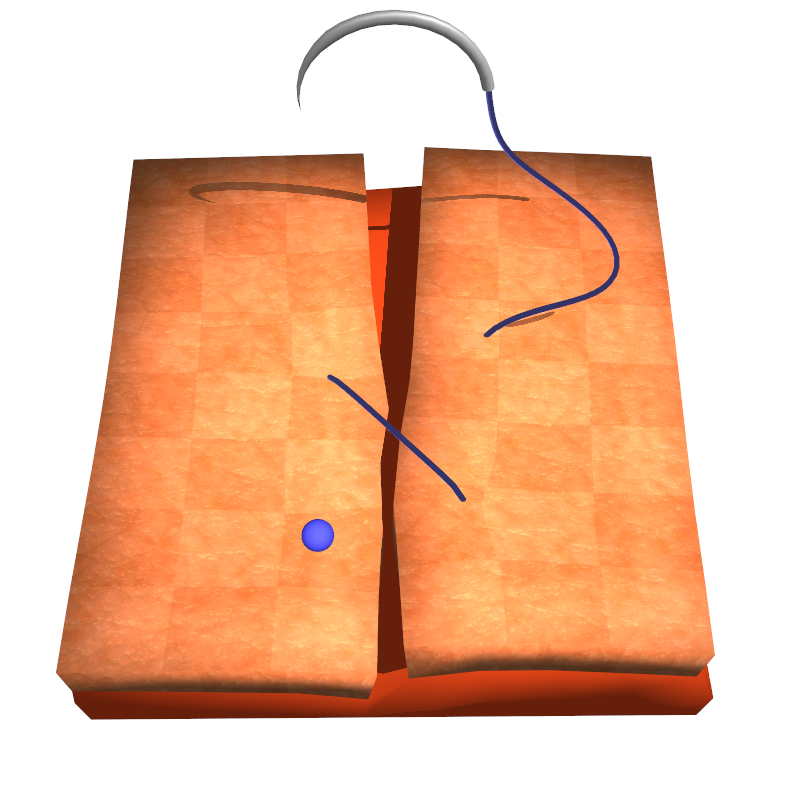
\includegraphics[width=4cm]{IMG/FrictionConstraint2.png}
   \caption{When we stop to pull on the thread, the suture point is opening again (left). Thanks to dry friction model, the suture point is maintained closed (right).}
\label{fig:friction}
\end{center} 
\end{figure}

By integrating friction in our approach we can simulate realistic scenarios. For instance it is well known by surgeons that a braided suture has a higher friction than a monofilament suture, as their friction coefficients $\mu$ are different. Indeed, to overcome static friction and advance the thread, the interaction force applied needs to reach the threshold $\mu . p$, where $p$ is the pressure exerted by the tissue onto the thread. This pressure is currently estimated from the stiffness of the soft tissue and is considered constant throughout the whole simulation. 

The friction resistance is given by the graph in Fig. (\ref{fig:friction2}). In comparison to the Coulomb's model of friction, we added a damping coefficient $\alpha$ to the dynamic friction, similar to the Karnopp friction model \cite{Karnopp}.
We then integrate $r$ along the part of the needle-thread curve that has been inserted into the tissue. As we sample the constraints along the insertion path, we distribute each friction constraint locally along the needle-thread curve to compute the friction force: $\lambda=l \pi d . r$, with $l$ the length of the curve part and $d$ the diameter of the cross-section.

\begin{figure}[ht]
\begin{center} 
   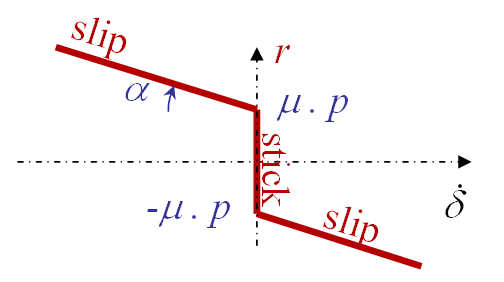
\includegraphics[width=7cm]{IMG/friction.png}
   \caption{Graph of the friction law used to constraint the motion of the needle and the thread inside the tissue.}
\label{fig:friction2}
\end{center} 
\end{figure}


\subsection{Contact}
\label{sec:contact}

%% commentaire: l�, il faudrait peut-�tre un peu moins rentrer dans les d�tails en citant d'autres papiers: la r�solution du contact par contrainte de compl�mentarit� a d�j� �t� trait� � de nombreuses reprises (Baraff, ...)
%In the following sections, we do not make any assumption over the choice of a collision detection method as our approach is independant of the method used for the collision detection. The violation $\delta$ is seen as a measure of interpenetration depth between two objects in contact. This measure can be obtained by discrete collision detection techniques, continuous collision detection techniques or proximity detection approaches.

During a simulation of a suturing task, contacts may occur at different locations (see Fig. \ref{contacts}). In all instances the contacts need to be modeled accurately to depict the real nature of the interaction, while remaining compatible with real-time simulation.

\begin{figure}[htbp]
\centering
   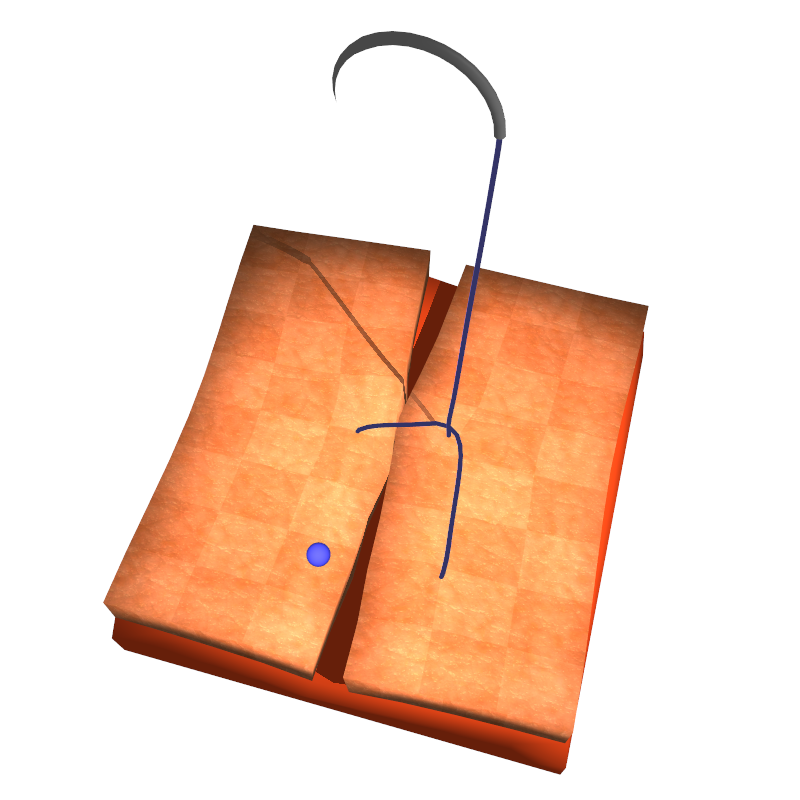
\includegraphics[width=6.5cm]{IMG/AutoCollisConstraint.png}
   \caption{Examples of contacts occuring during suture: contact between the soft tissue walls, between the soft tissue and the thread and autocollision of the suture thread.}
\label{contacts}
\end{figure}

Contact constraints prevent objects from interpenetration. $\delta_c$ is then a  measure of interpenetration depth between two objects in contact. This measure can be obtained by discrete collision detection techniques, continuous collision detection techniques or proximity detection approaches.
Contact is inherently a unilateral constraint, in the sense that it corrects the interpenetration of two objects, but will not make them stick back to each other after they have been separated. 
This unilateral law can be written $0 \leq \delta_c \perp \lambda_c \geq 0$. Assuming the \textit{compliance law} is known, the resolution is trivial:
if $-\delta_0  \mathbf{W}^{-1}  \geq 0$, $\lambda_c = -\delta_0 \mathbf{W}^{-1}$, 
else $\lambda_c = 0$.


%The law describing these constraints is non-smooth and has been introduced by Signorini. For the constraint to be verified, if the two objects are in contact we want the penetration distance $\delta_c$ to be null so the interaction force $\lambda$ is necessarily positive in the direction of the surface nomal ($\delta_c = 0$, $\lambda \geq 0$). On the contrary, when the points we consider are not penetrating $\delta_c$ is positive and the interaction force is null ($\delta_c \geq 0$, $\lambda = 0$).

For realistic simulation of both needle driving and thread insertion through the tissue, we add friction constraints along the tangential directions of the contact. In our approach we consider dry friction, and use the well known Coulomb's friction law. For this friction constraint, $\delta$ measures the relative motion in the tangential space. The resolution of the constraint is explained by Fig. \ref{coulomb}.

\begin{figure}[htbp]
\centering
   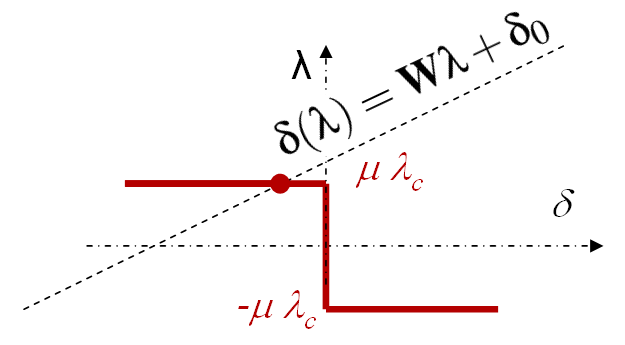
\includegraphics[width=7cm]{IMG/Coulomb.png}
   \caption{\textbf{Coulomb's law} is depicted in red and depends on the value found for $\lambda_c$ and on a friction coefficient $\mu$. If the compliance law is known, it can be represented on the graph by a line. The solution is the given by the intersection of this line with the Coulomb's law.}
\label{coulomb}
\end{figure}

One important point is that we do not know beforehand the direction of the lateral motion for the contact constraints. We then have to update friction direction multiple times as the computation goes on. Several papers discuss this problem, for instance see \cite{Baraff91}.



\subsection{Constraints on embedded Points}~\label{sec:embed}
\CD{In the previous paper, this section was before..}
Applying constraints on arbitrary points within a volume or surface mesh is critical, as it removes the reliance on dynamically remeshing often required by other methods.

Two complementary steps are necessary. First, we need to be able to update the point position given new positions of the mesh vertices. Then, forces applied by the constraint solver to the embedded point must be converted to equivalent forces applied to the vertices. Observing the virtual work principle, this can be done with a projection as explained below, following the same proof as used in~\cite{NKJF09} for penalty forces.

Given the current positions of the mesh vertices, we can compute a matrix $H_x$ denoting the linear relation between a small displacement $u$ of the embedded constraint point $x$ and the displacement $U$ of the mesh vertices :
\begin{equation}
u = \mathbf{H}_x U
\label{eq:Hx}
\end{equation}
In finite elements, $\mathbf{H}_x$ simply consists of the shape functions evaluated at $x$. In the case of a simple linear embedding, this matrix is constituted by the barycentric coordinates of $x$ within the containing tetrahedron or hexahedron.

Given a force $f$ to be applied to the embedded point, we need to compute the equivalent forces $F$ applied to the mesh vertices.
To be equivalent, these forces must create the same work, that is, $U^T F = u^T f$. Using equation \ref{eq:Hx}, 
we obtain $U^T F = u^T \mathbf{H}_x^T f$. In order for this relation to be true for any given small displacement $u$, the equivalent force is necessarily
\begin{equation}
     F = \mathbf{H}_x^T f.
\end{equation}
This relation holds for all possible embeddings.

%\subsection{Constraint Space}
The constraint models presented in section \ref{sec:constraints} are  described using a law which links a distance measure $\delta$ to a force $\lambda$.
These values, provided in the \textit{constraint space}, have now to be mapped with the relative displacements and the forces of the deformable models in the \textit{motion space}.
%Our constraints are described in the \textit{constraint space} which is a generalization of the \textit{contact space} introduced by Ruspini \textit{et al.}~\cite{Ruspini}. Writing constraint laws in this space is often easier than it would be in the motion space. %We link the positions in the motion space to the constraints space using a mapping function.

When a constraint $i$ is attached to a given point $x$, a vector $n_x$ (corresponding to the surface normal at the contact point for instance) maps a motion in space to a variation of the constraint value $\mathbf{\delta}_i$. After solving the constraints we obtain a response force $\mathbf{\lambda}_i$. Using the same virtual work principle as above, this force can be mapped to the point in motion space by $f_x = n_x^T \mathbf{\lambda}_i$.
Therefore, we can compute the final sparse matrix $\mathbf{H}$ linking the \textit{constraint space} and \textit{motion space} as $f = \mathbf{H}^T \mathbf{\lambda}$, where each row $i$ of $\mathbf{H}$ can be computed as
\begin{equation}
\mathbf{H}_i = n_x\mathbf{H}_x \quad \forall \textrm{ point } x \textrm{ used by constraint } i
\end{equation}
%where $\mathbf{H}_x$ is the matrix linking the point $x$ to the mesh vertices (see section~\ref{sec:embed}).



%%%%%%%% %%%%%%%%%%%
%%  SECTION : Tissue-suture interaction   %%
%%%%%%%% %%%%%%%%%%%

\section{Tissue-suture interaction}
Motivations: accurate coupling between suture model and soft-tissues, find a solution that computes constraint solution, fast-computation needed !
Solutions: Use of compliance measure within implicit framework. For each model (suture / soft-tissue), the computation of the compliance is optimized differently.

Introduction of the coupling equations

\subsection{Compliance of the soft-tissue}

\CD{Precomputed ou Preconditionner ?}


\subsection{Compliance of the suture}

\CD{TODO ! }

Principle: The BTD solver allows for very fast computation of the wire-like structure because it relies on a very sparse matrix.
However, the compliance is not sparse at all....

The approach is based on the same technique than in \CD{Miccai paper 2004}.
However, we have generalized the approach to deal with self-collision problem.

\subsection{Partially assembled Gauss-Seidel solver}

Motivation: Heterogeneous constraints + need of a fast solver...
 
 \subsection{Haptic Rendering}



%%%%%%%% %%%%%%%%%%%
%%  SECTION : Results   %%
%%%%%%%% %%%%%%%%%%%
\section{Results}


%%%%%%%% %%%%%%%%%%%
%%  SECTION : Conclusion   %%
%%%%%%%% %%%%%%%%%%%
\section{Conclusion}

\section*{Acknowledgements}

To Robert, for all the bagels.

\bibliographystyle{acmsiggraph}
\bibliography{Biblio}
\end{document}
